% ============================================================================
% TP6 -- Medición con punta de corriente (entregable OE7)
% Plantilla basada en el TP1 (RE-TP-001). Un solo archivo .tex. Necesita en la
% misma carpeta: logo_fiuba.png, logo_materia.png y la carpeta Imagenes.
% Los gráficos de Zt se generan con graficos_zt.py a partir de TP6_Zt_puntas.xlsx.
% Compilar con pdfLaTeX (Overleaf: Menu > Compiler > pdfLaTeX).
% ============================================================================
\documentclass[11pt,a4paper]{article}

\usepackage[utf8]{inputenc}
\usepackage[T1]{fontenc}
\usepackage[default]{sourcesans}
\usepackage[spanish,es-tabla,es-nodecimaldot]{babel}
\usepackage[a4paper,margin=2.5cm,headheight=14pt]{geometry}
\usepackage{graphicx}
\usepackage{float}       % permite la opcion [H] en figuras y tablas
\usepackage{booktabs}
\usepackage{array}
\usepackage{longtable}
\usepackage{enumitem}
\usepackage{amsmath}
\usepackage{xcolor}
\usepackage{fancyhdr}
\usepackage{tikz}
\usetikzlibrary{babel}   % evita el choque entre TikZ y los atajos < > del español
\usetikzlibrary{positioning}
\usepackage[hidelinks]{hyperref}

% ---------------------------------------------------------------- datos ----
\newcommand{\codigo}{OE7}
\newcommand{\version}{0.1 (borrador)}
\newcommand{\fecha}{30 de octubre de 2026}

% Texto que hay que completar o confirmar antes de usar el documento
\newcommand{\pendiente}[1]{\textcolor{red}{[#1]}}

\pagestyle{fancy}
\fancyhf{}
\lhead{\small \codigo{}, Medición con punta de corriente}
\rhead{\small Versión \version}
\cfoot{\small \thepage}

\setlist{itemsep=2pt,topsep=4pt}

\begin{document}

% ============================================================== caratula ====
% numeracion aparte en la caratula para que no repita el ancla page.1 de hyperref
\pagenumbering{alph}
\begin{titlepage}
  \centering
  \vspace*{0.5cm}
  % logo de la facultad a la izquierda y logo de la materia a la derecha
  \begin{minipage}[c]{0.56\textwidth}
    \centering
    
\includegraphics[width=\textwidth]{logo_fiuba.png}
  \end{minipage}\hfill
  \begin{minipage}[c]{0.34\textwidth}
    \centering
    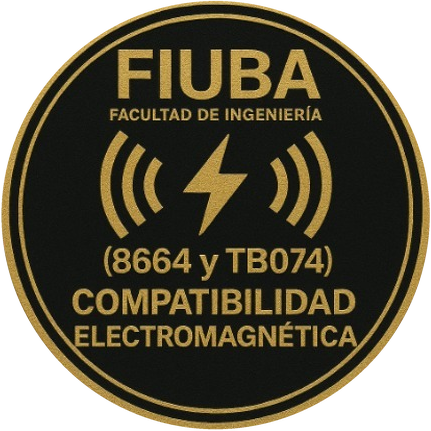
\includegraphics[width=\textwidth]{logo_materia.png}
  \end{minipage}\par
  \vspace{0.8cm}
  {\large Universidad de Buenos Aires, Facultad de Ingeniería\par}
  {\large Compatibilidad Electromagnética (8664 y TB074)\par}
  {\large Trabajo Práctico N.\textsuperscript{o}~6, Entregable OE7\par}
  \vspace{1.6cm}
  {\LARGE \bfseries Medición con punta de corriente\par}
  \vspace{0.6cm}
  {\Large Caracterización de la impedancia de transferencia\par}
  \vspace{0.8cm}
  {\large Código: \textbf{\codigo}\par}
  \vfill
  \begin{tabular}{ll}
    \toprule
    Autores             & Martín Ledesma \\
                        & Alejandro Catonar \\
    Docentes            & Pablo Marino Belcaguy \\
                        & Walter Gustavo Fano \\
    Fecha               & \fecha \\
    \bottomrule
  \end{tabular}
  \vspace{1cm}
\end{titlepage}
\pagenumbering{arabic}

\tableofcontents
\newpage

% ============================================================================
\section{Introducción}

\subsection{Cómo funciona una punta de corriente}

Una punta de corriente es un transformador de corriente. El cable que se quiere medir pasa por el centro de un núcleo de ferrita y hace de primario. Sobre el núcleo hay un bobinado secundario que se conecta a un instrumento con entrada de 50~$\Omega$, por ejemplo un analizador de espectro. Así se mide la corriente sin cortar el cable, y por eso en EMC se usa para medir las corrientes de modo común que circulan por los cables~[\ref{ref:paul}].

La punta se describe con su impedancia de transferencia $Z_t$, que es la tensión a la salida de la punta sobre la corriente en el conductor:
\begin{equation}
  Z_t = \frac{V_2}{I_1}
\end{equation}
Se suele dar en dB$\Omega$. Con $Z_t$ conocida, la corriente sale directo de la lectura del analizador:
\begin{equation}
  I\,(\mathrm{dB\mu A}) = V\,(\mathrm{dB\mu V}) - Z_t\,(\mathrm{dB\Omega})
\end{equation}
En baja frecuencia $Z_t$ crece unos 20~dB por década. Después tiene una zona plana, que es donde conviene usar la punta, y a frecuencias altas aparecen resonancias del bobinado y del núcleo que la deforman.

\subsection{Importancia de un \textit{JIG} normalizado}

Para medir $Z_t$ hay que hacer pasar por la punta una corriente conocida. La norma CISPR 16-1-2 usa un \textit{JIG} coaxial adaptado a 50~$\Omega$, de modo que la corriente se calcula a partir de la tensión sobre la carga de 50~$\Omega$~[\ref{ref:cispr}]. La norma ISO 11452-4 pide además que el \textit{JIG} tenga una ROE menor a 1,2. Si el \textit{JIG} no está bien adaptado aparecen reflexiones, la corriente real deja de ser la que se supone y el resultado cambia de un laboratorio a otro~[\ref{ref:sekiguchi}]. El problema es que estos \textit{JIG} son caros y muchos fabricantes no los venden.

\subsection{Objetivo}

Medir la impedancia de transferencia de dos puntas de corriente caseras con un montaje más sencillo que un \textit{JIG} normalizado. Se usa un lazo de dos cables lo más corto posible, mucho menor que la longitud de onda, tomado de~[\ref{ref:paper}]. Se busca ver si el método da resultados útiles y si es repetible, comparando dos corridas hechas en días distintos.

% ============================================================================
\section{Equipos y montaje}

\begin{table}[H]
  \centering
  \begin{tabular}{@{}llp{6.2cm}@{}}
    \toprule
    Equipo & Modelo & Detalle \\
    \midrule
    Generador de RF & RIGOL DSG830 & 9~kHz a 3~GHz, usado en 0~dBm \\
    Analizador de espectro & Siglent SSA3032X & 9~kHz a 3,2~GHz \\
    Cable de alimentación del lazo & RG58 & 75~cm \\
    Cable de la punta al analizador & RG213 & 1~m \\
    Carga & Sin modelo & 50~$\Omega$ con conector BNC \\
    Punta circular & Casera & Etiqueta 10~kHz a 90~MHz, $Z_t$ desde $-22$~dB$\Omega$ \\
    Punta cuadrada con apertura & Casera & Etiqueta 10~kHz a 90~MHz, $Z_t$ de $-27$ a 10~dB$\Omega$ \\
    \bottomrule
  \end{tabular}
  \caption{Equipos usados.}
  \label{tab:equipos}
\end{table}

El generador alimenta un cable RG58. En su extremo el vivo y la malla se separan en dos cables, uno rojo y uno negro, que forman un tramo de unos 10~cm con unos 5~cm entre ellos. El cable rojo pasa por el centro de la punta, sostenido con espuma para que quede centrado, y llega al vivo de un conector BNC de chasis. El negro se une al cuerpo del mismo conector con un cocodrilo, y en ese conector va la carga de 50~$\Omega$. La salida de la punta va al analizador por el RG213. La figura~\ref{fig:esquema} muestra el esquema y las figuras~\ref{fig:banco} a~\ref{fig:puntas} muestran el banco.

\begin{figure}[H]
  \centering
  \begin{tikzpicture}[caja/.style={draw, rounded corners, minimum height=1cm, minimum width=2.6cm, align=center, font=\small}, node distance=1.6cm]
    \node[caja] (gen) {Generador\\DSG830};
    \node[caja, right=of gen] (lazo) {Lazo con\\punta de corriente};
    \node[caja, right=of lazo] (carga) {Carga\\50~$\Omega$};
    \node[caja, below=1.2cm of lazo] (sa) {Analizador\\SSA3032X};
    \draw[->, thick] (gen) -- node[above, font=\footnotesize] {RG58} (lazo);
    \draw[->, thick] (lazo) -- (carga);
    \draw[->, thick] (lazo) -- node[right, font=\footnotesize] {RG213, 1~m} (sa);
  \end{tikzpicture}
  \caption{Esquema del montaje.}
  \label{fig:esquema}
\end{figure}

\begin{figure}[H]
  \centering
  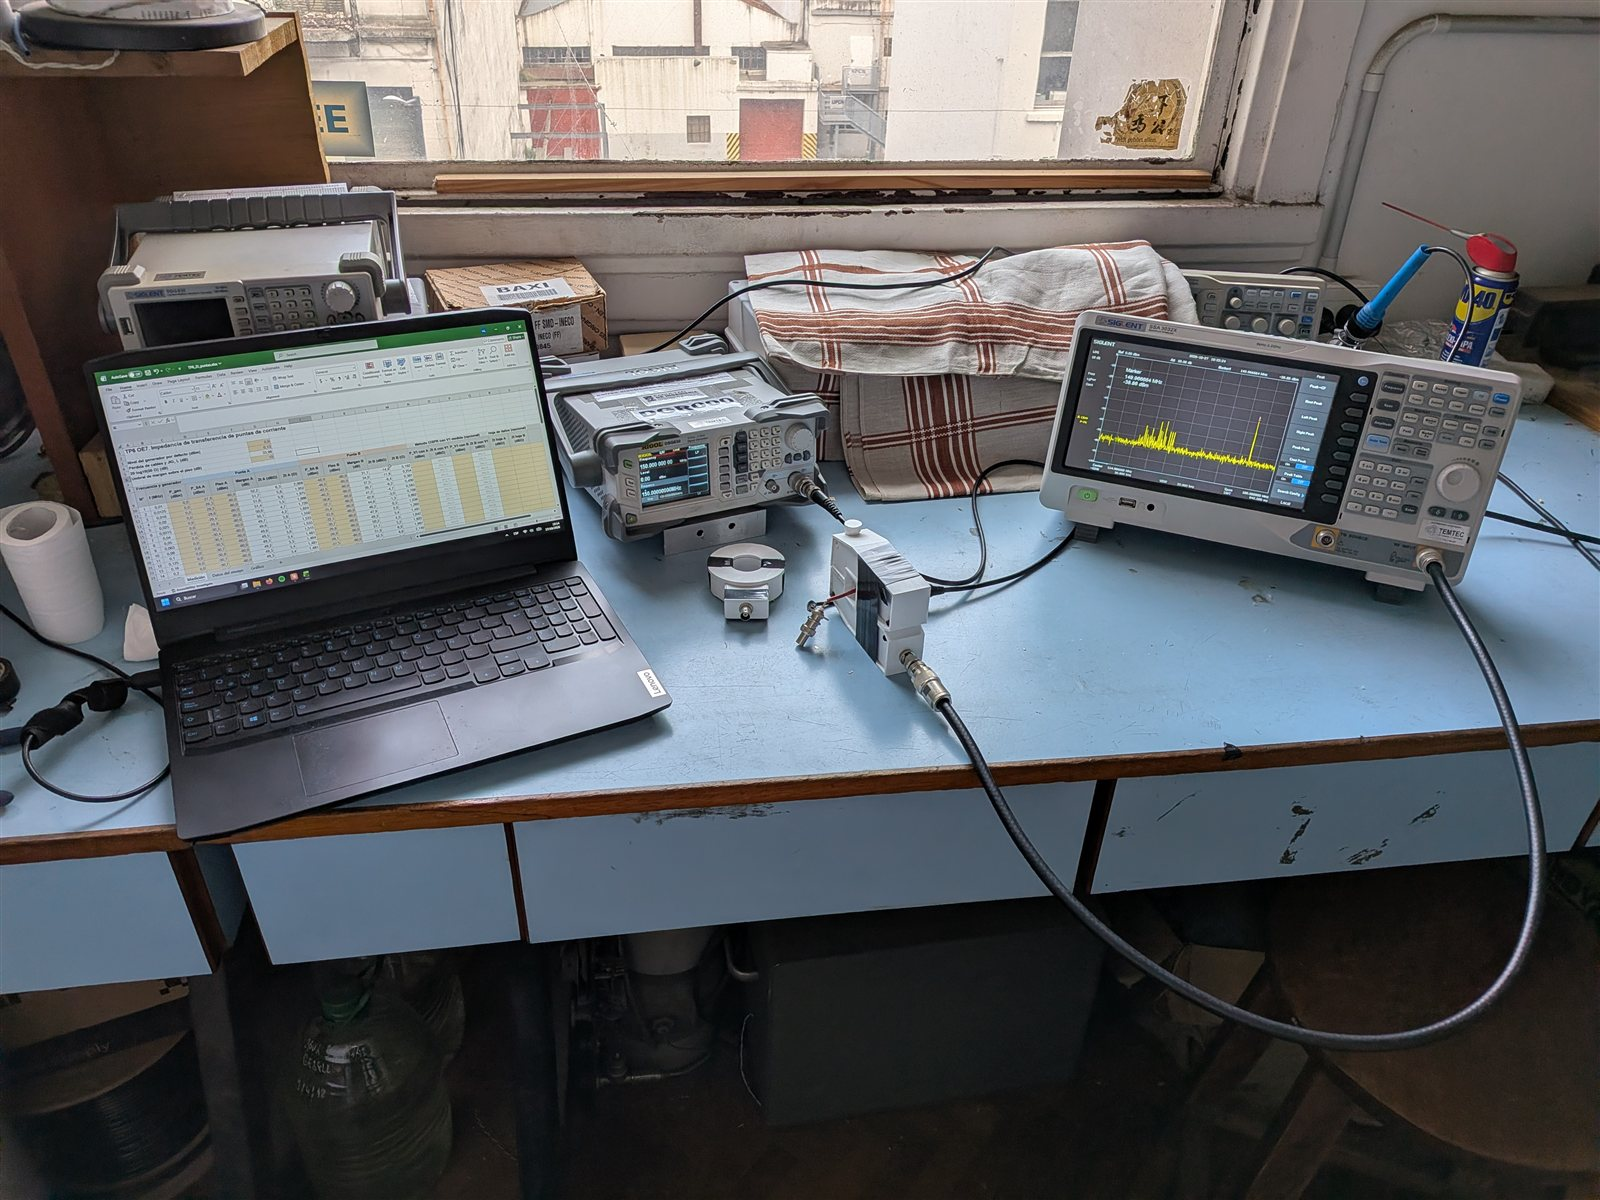
\includegraphics[width=0.95\textwidth]{Imagenes/banco.jpg}
  \caption{Banco de trabajo con el generador, el analizador y el lazo.}
  \label{fig:banco}
\end{figure}

\begin{figure}[H]
  \centering
  % misma altura para que las dos fotos queden como mosaico
  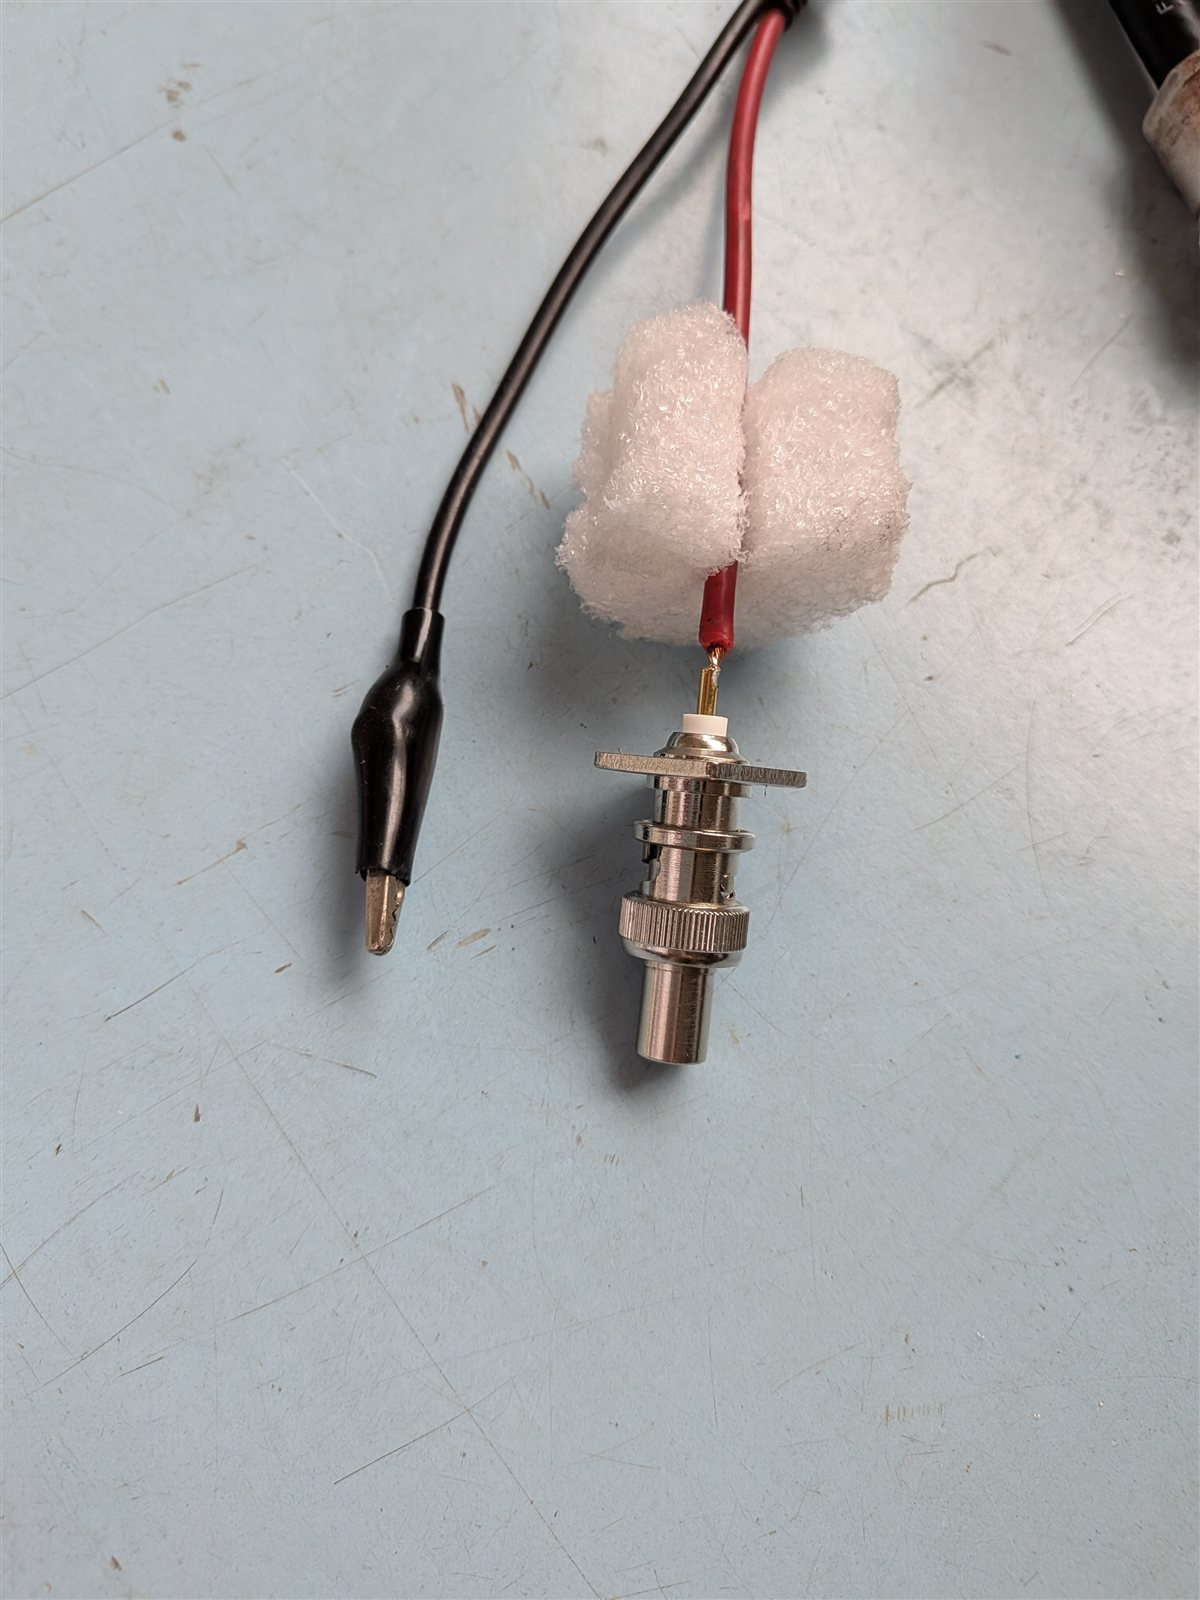
\includegraphics[height=7.2cm]{Imagenes/lazo.jpg}\hfill
  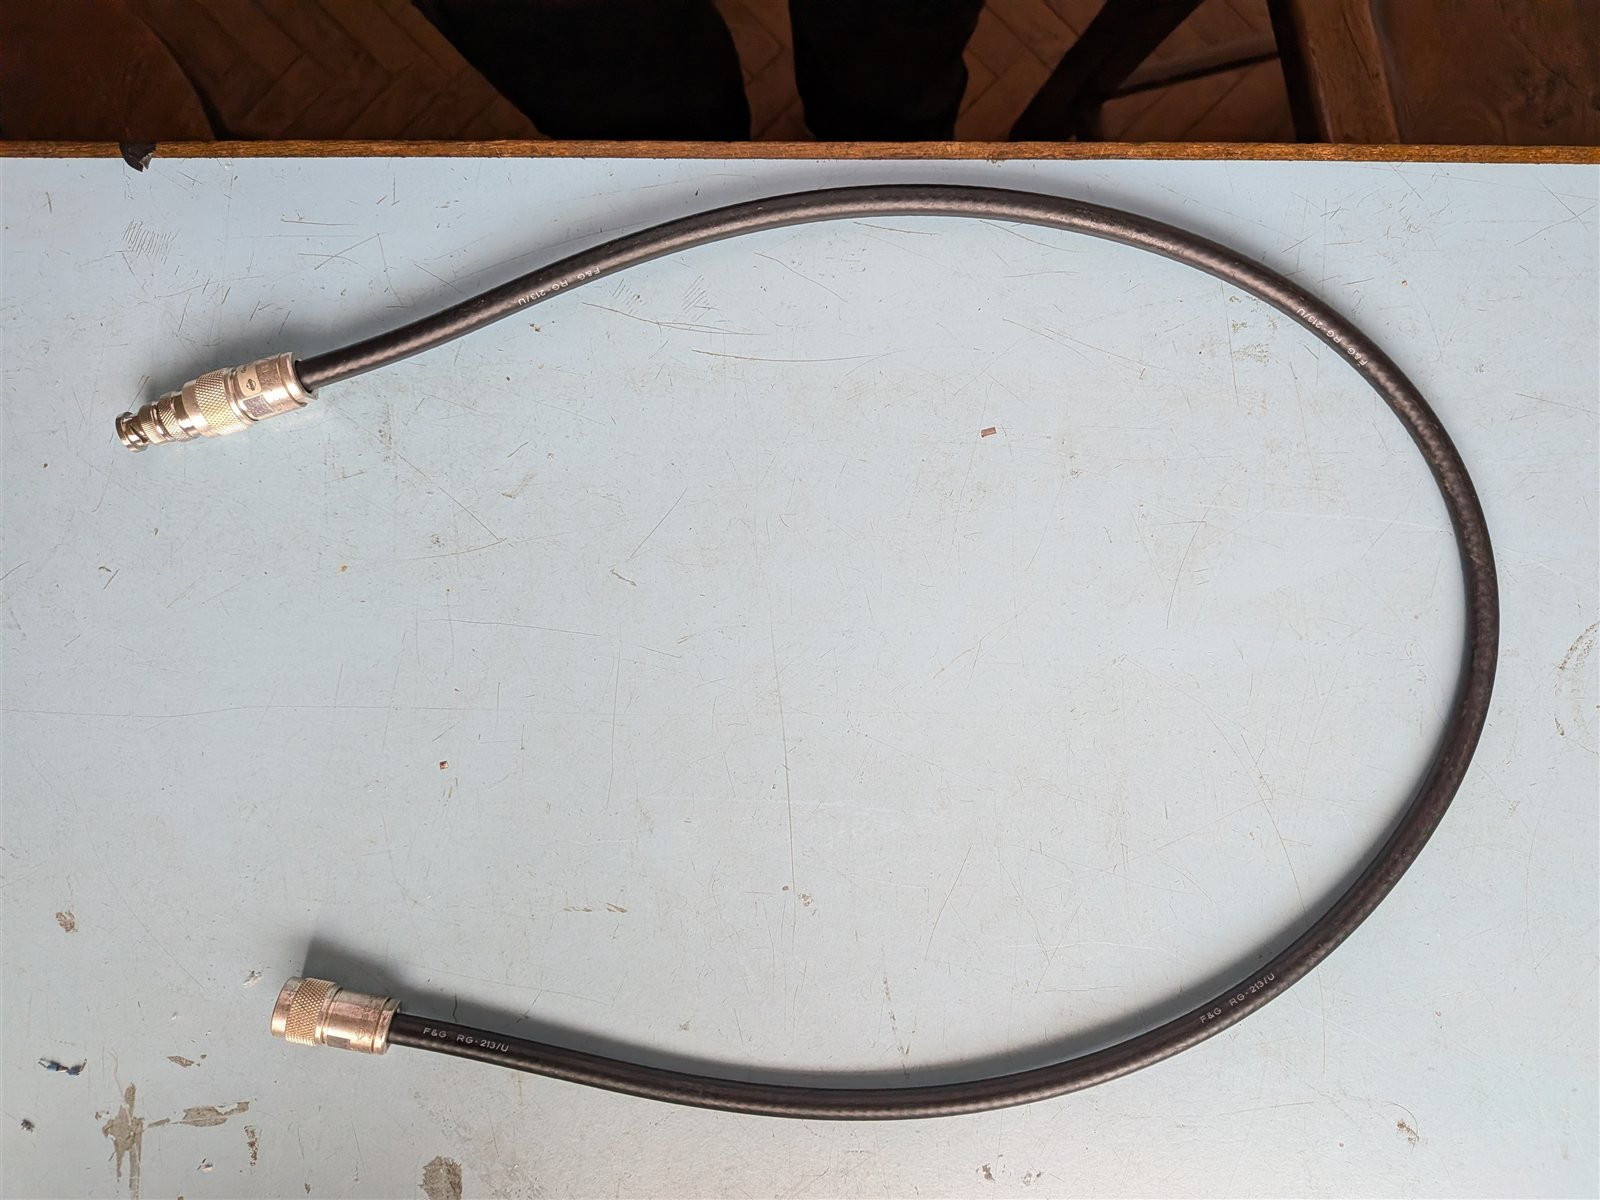
\includegraphics[height=7.2cm]{Imagenes/cable_rg213.jpg}
  \caption{Extremo del lazo con el conector BNC de chasis (izquierda) y cable RG213 de 1~m (derecha).}
  \label{fig:lazo}
\end{figure}

\begin{figure}[H]
  \centering
  \begin{minipage}[c]{0.48\textwidth}
    \centering
    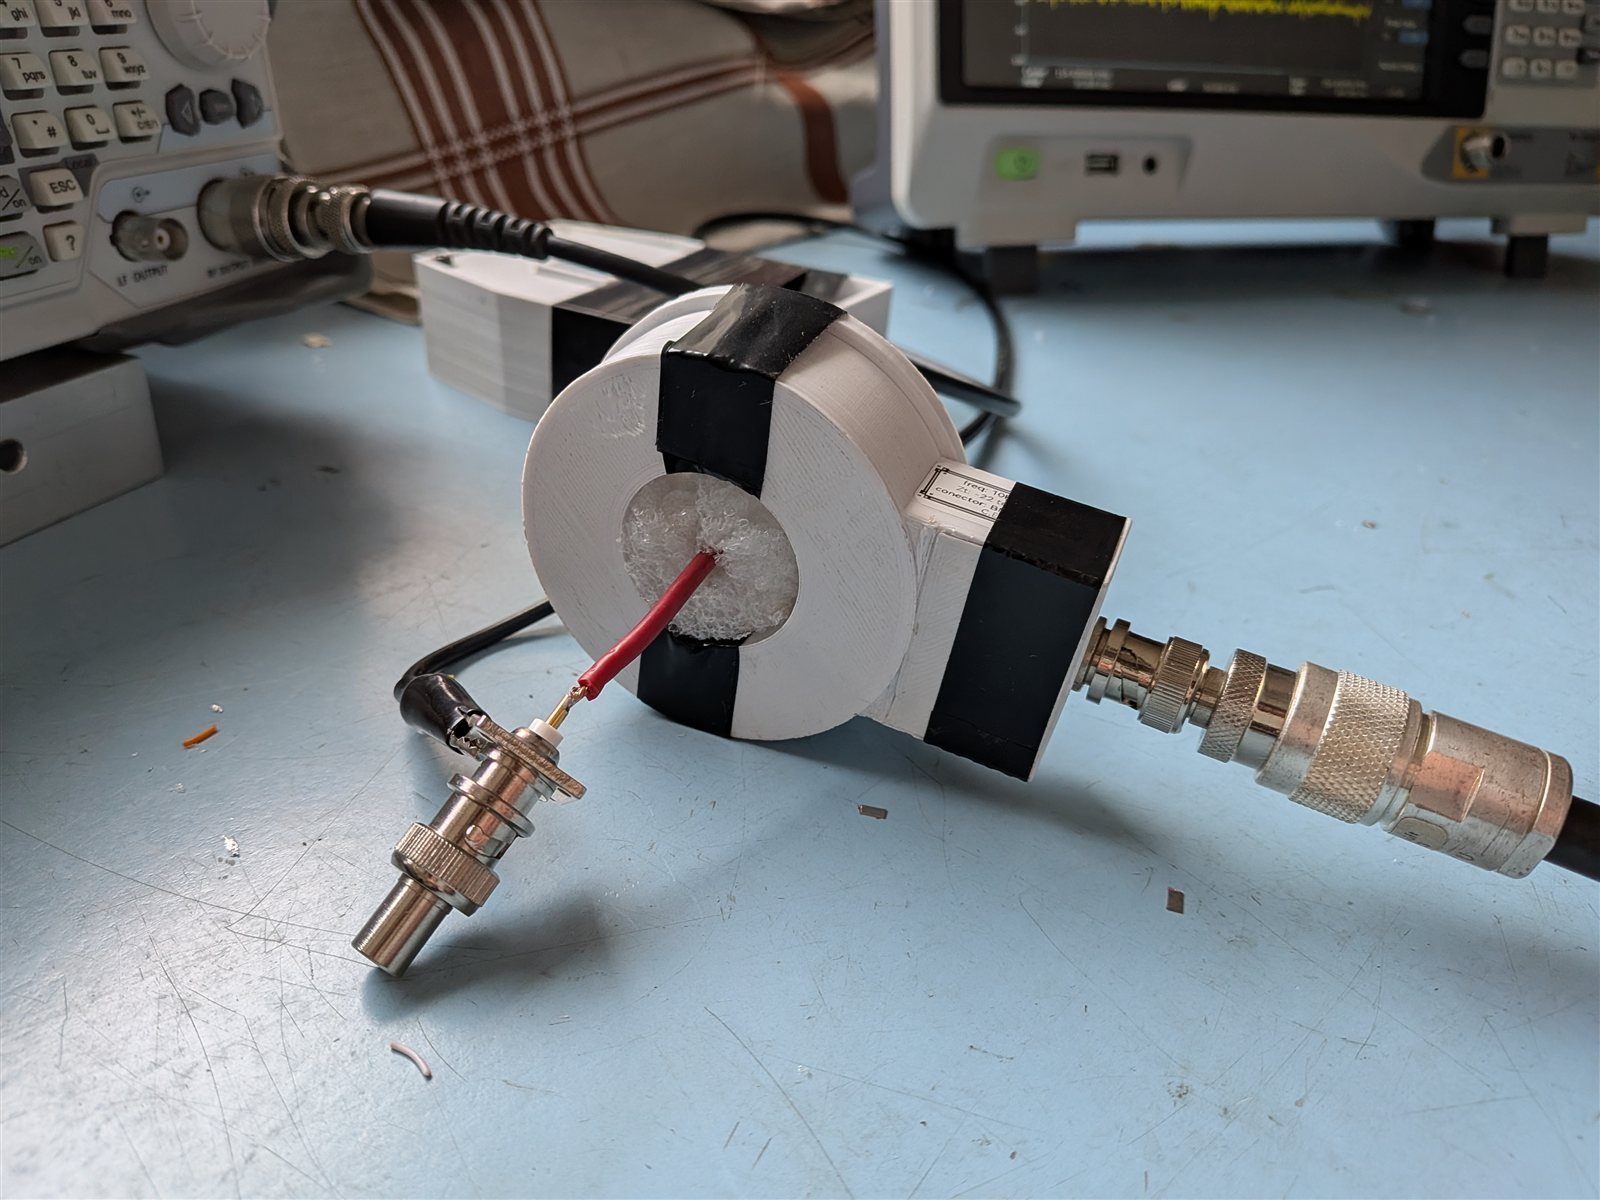
\includegraphics[width=\textwidth]{Imagenes/lazo_punta_circular.jpg}
  \end{minipage}\hfill
  \begin{minipage}[c]{0.48\textwidth}
    \centering
    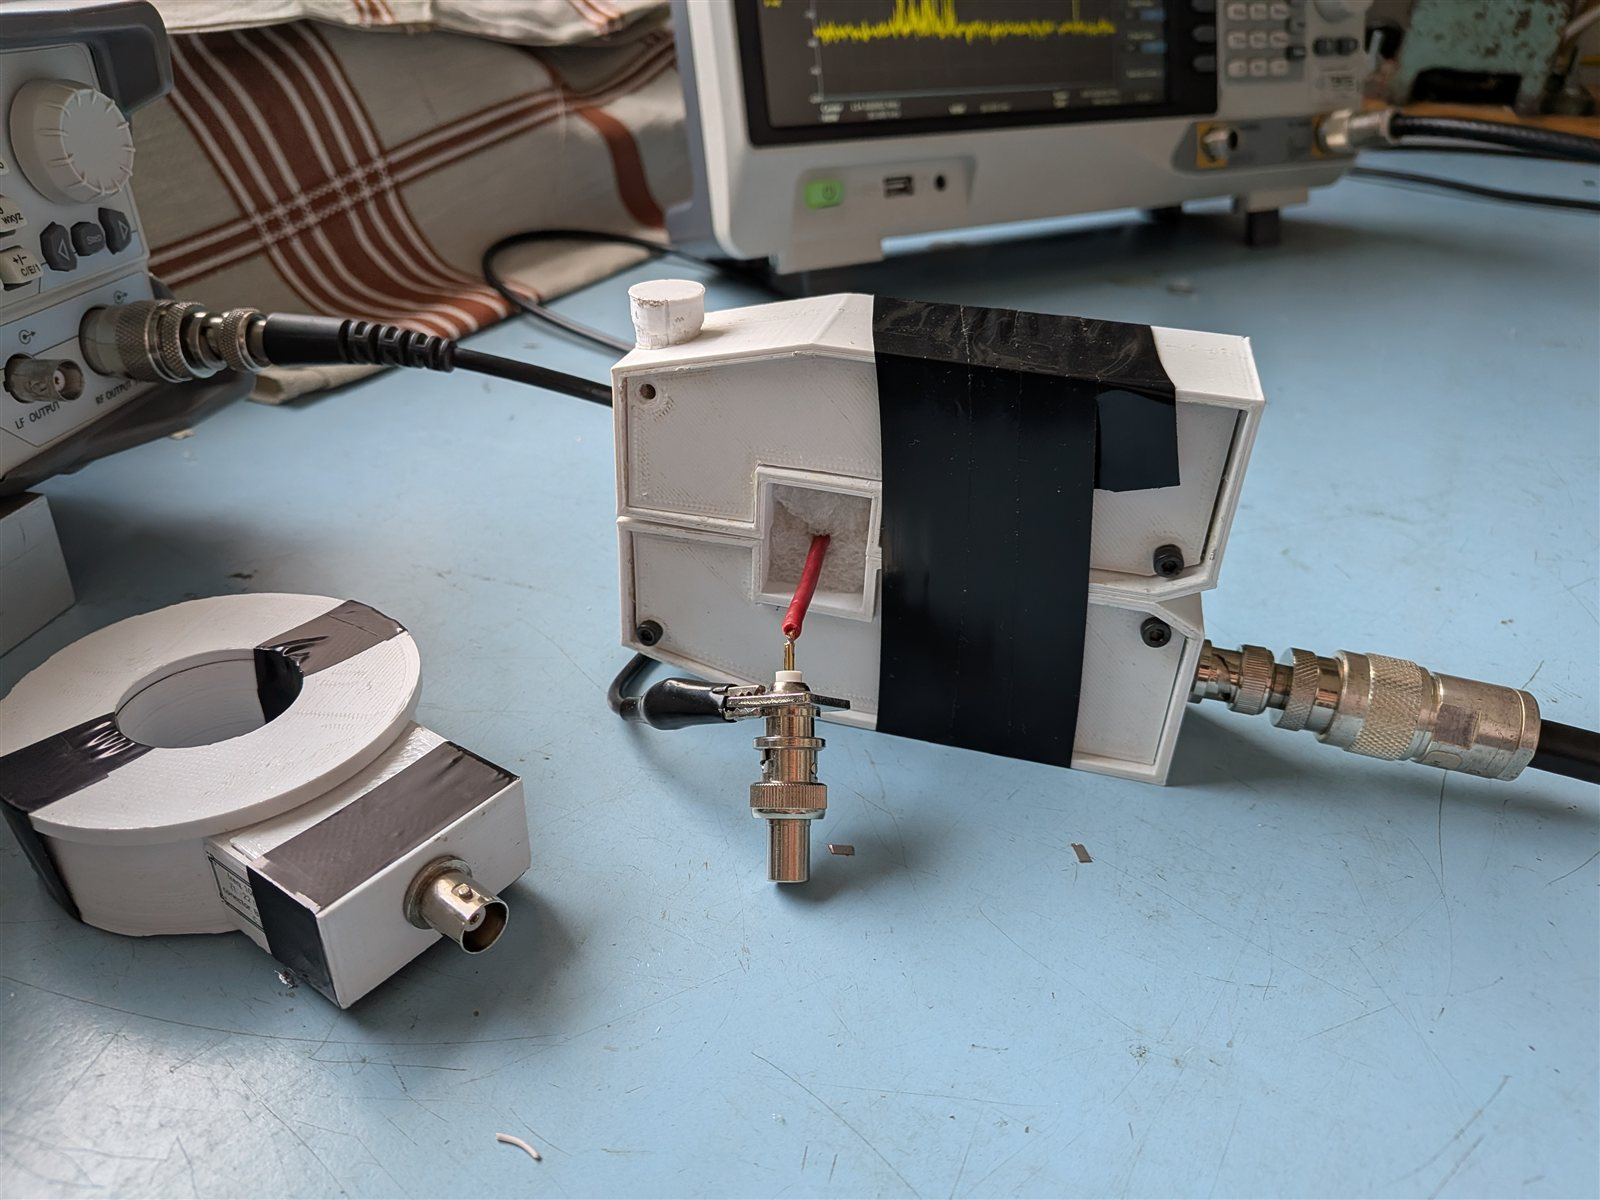
\includegraphics[width=\textwidth]{Imagenes/lazo_punta_cuadrada.jpg}
  \end{minipage}
  \caption{Punta circular (izquierda) y punta cuadrada con apertura (derecha) montadas en el lazo.}
  \label{fig:puntas}
\end{figure}

% ============================================================================
\section{Procedimiento}

\begin{enumerate}
  \item Armar el lazo y fijar la punta con cinta en el punto medio del tramo, con el cable rojo centrado. La punta no se mueve durante toda la medición.
  \item Poner el generador en 0~dBm, sin modulación. Debajo de 100~kHz el DSG830 entrega como máximo +5~dBm, así que 0~dBm sirve para todo el rango.
  \item Configurar el analizador con nivel de referencia de 0~dBm, atenuación de 20~dB y preamplificador apagado. De 9~kHz a 1~MHz se usa RBW y VBW de 100~Hz con span de 100~kHz. De 1 a 150~MHz se usa RBW y VBW de 100~kHz con span de 100~MHz.
  \item En cada frecuencia leer el pico con el marcador. Esa lectura es $P_{SA}$.
  \item Apagar la salida del generador y leer el piso en la misma frecuencia.
  \item Repetir con la otra punta. Repetir todo otro día para la segunda corrida.
\end{enumerate}

Se midieron 55 frecuencias entre 10~kHz y 150~MHz. Hasta 20~MHz se usa la serie R10 (10 puntos por década) y de 20 a 90~MHz la serie R20, más densa porque ahí la respuesta cambia más. Se agregaron 58, 60 y 62~MHz para mirar mejor un salto que aparece en esa zona, y 100, 112, 125, 140 y 150~MHz para ver qué pasa por encima del rango declarado.

\subsection{Cálculo de la impedancia de transferencia}

Si el lazo está adaptado, la corriente por el lazo y la tensión a la salida de la punta salen de las potencias del generador y del analizador:
\begin{equation}
  I = \sqrt{\frac{P_{gen}}{50~\Omega}} \qquad V = \sqrt{P_{SA} \cdot 50~\Omega}
  \qquad \Rightarrow \qquad Z_t = \frac{V}{I} = 50~\Omega \cdot \sqrt{\frac{P_{SA}}{P_{gen}}}
\end{equation}
Pasado a decibeles queda:
\begin{equation}
  Z_t\,(\mathrm{dB\Omega}) = P_{SA}\,(\mathrm{dBm}) - P_{gen}\,(\mathrm{dBm}) + 20\log_{10}(50) + L
\end{equation}
donde $20\log_{10}(50) = 34{,}0$~dB y $L = 0{,}13$~dB es la pérdida del RG213 de 1~m con sus conectores, tomada de la hoja de datos del cable en el peor caso (150~MHz). Es el mismo cálculo de CISPR 16-1-2, con la diferencia de que se usa el nivel que indica el generador en lugar de medir la tensión sobre la carga.

% ============================================================================
\section{Resultados}

Las figuras~\ref{fig:zt_circular} y~\ref{fig:zt_cuadrada} muestran $Z_t$ de cada punta en la primera corrida. La figura~\ref{fig:zt_circular_util} repite la punta circular solo en su rango útil, con la escala vertical ampliada para ver mejor la zona plana. \pendiente{Sumar la corrida 2 a los gráficos.} En todas las frecuencias la señal quedó por lo menos 26~dB por encima del piso, así que el ruido no afecta las lecturas.

\begin{figure}[H]
  \centering
  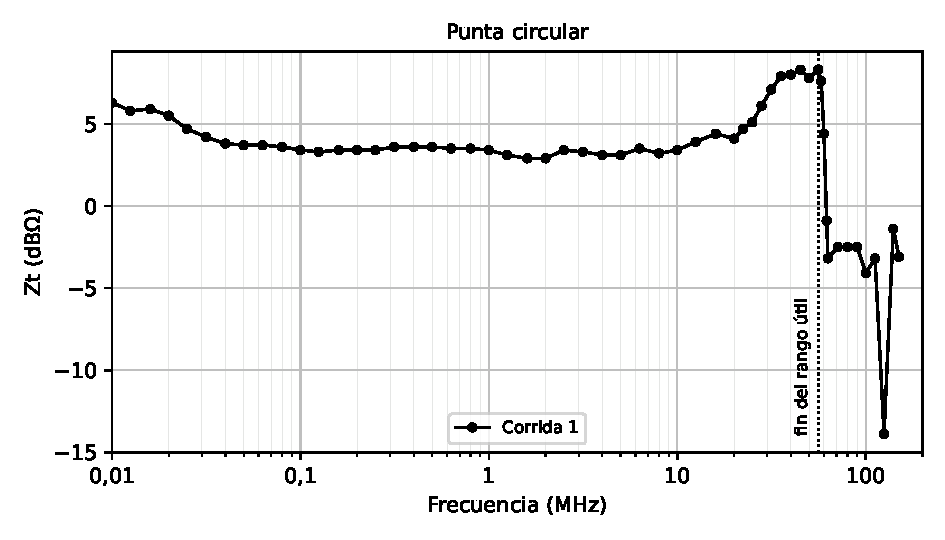
\includegraphics[width=0.9\textwidth]{Imagenes/zt_punta_circular.pdf}
  \caption{Impedancia de transferencia de la punta circular.}
  \label{fig:zt_circular}
\end{figure}

\begin{figure}[H]
  \centering
  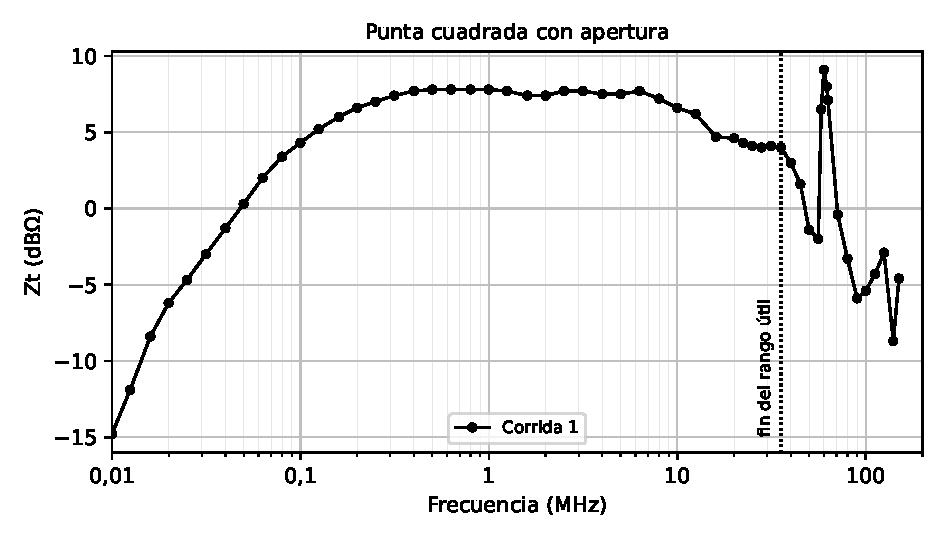
\includegraphics[width=0.9\textwidth]{Imagenes/zt_punta_cuadrada.pdf}
  \caption{Impedancia de transferencia de la punta cuadrada con apertura.}
  \label{fig:zt_cuadrada}
\end{figure}

\begin{figure}[H]
  \centering
  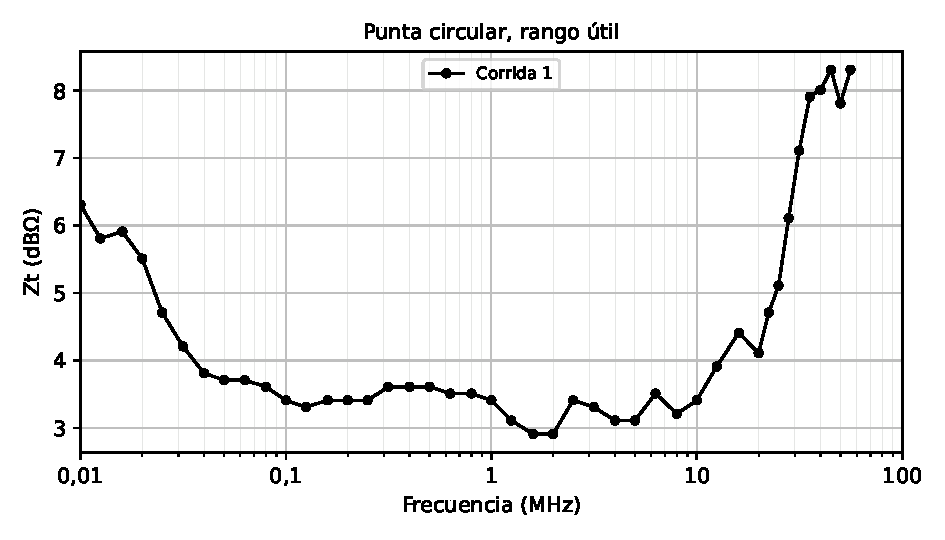
\includegraphics[width=0.9\textwidth]{Imagenes/zt_punta_circular_rango_util.pdf}
  \caption{Impedancia de transferencia de la punta circular dentro de su rango útil.}
  \label{fig:zt_circular_util}
\end{figure}

\subsection{Respuesta de cada punta}

\begin{itemize}
  \item La punta circular es casi plana entre 40~kHz y 20~MHz, con 3,5~dB$\Omega$ de promedio (1,5~$\Omega$) y valores entre 2,9 y 4,4~dB$\Omega$. Por debajo de 40~kHz sube hasta 6,3~dB$\Omega$ en 10~kHz. Entre 20 y 56~MHz sube hasta unos 8~dB$\Omega$. No muestra la subida de 20~dB por década dentro del rango medido, así que su zona de baja frecuencia estaría por debajo de 10~kHz.
  \item La punta cuadrada sube unos 20~dB por década desde 10~kHz, como un transformador de corriente común, y es plana de 250~kHz a 8~MHz, con 7,6~dB$\Omega$ de promedio (2,4~$\Omega$) y valores entre 7,0 y 7,8~dB$\Omega$. Desde 10~MHz baja de a poco hasta 4,0~dB$\Omega$ en 35,5~MHz, y desde 40~MHz cae más rápido.
  \item En la punta cuadrada los valores medidos quedan dentro del rango de $Z_t$ que indica la etiqueta, de $-27$ a 10~dB$\Omega$. \pendiente{Comparar la circular cuando se lea su etiqueta completa.}
\end{itemize}

\subsection{Rango útil}

Se toma como criterio que la punta funciona bien mientras cada punto queda cerca de sus vecinos, y que deja de funcionar cuando aparecen saltos grandes entre puntos cercanos. En la punta circular el primer salto aparece en 58~MHz, así que su rango útil llega hasta 56~MHz. En la cuadrada la curva empieza a caer más rápido desde 40~MHz y en 58~MHz aparecen saltos de casi 10~dB, así que su rango útil se toma hasta 35,5~MHz. Las dos quedan por debajo de los 90~MHz de la etiqueta. Los puntos entre 56 y 63~MHz se midieron varias veces, yendo y viniendo en frecuencia, y el salto se repitió igual, así que no es un error de lectura.

\begin{table}[H]
  \centering
  \begin{tabular}{@{}lllll@{}}
    \toprule
    Punta & Zona plana & $Z_t$ en la zona plana & Rango útil & Diferencia entre corridas \\
    \midrule
    Circular & 40~kHz a 20~MHz & 3,5~dB$\Omega$ (1,5~$\Omega$) & 10~kHz a 56~MHz & \pendiente{corrida 2} \\
    Cuadrada & 250~kHz a 8~MHz & 7,6~dB$\Omega$ (2,4~$\Omega$) & 10~kHz a 35,5~MHz & \pendiente{corrida 2} \\
    \bottomrule
  \end{tabular}
  \caption{Resumen de resultados.}
  \label{tab:resumen}
\end{table}

\subsection{Falla de las dos puntas cerca de 60~MHz}

Las dos puntas fallan en frecuencias muy cercanas, entre 56 y 62~MHz, lo que hace sospechar del montaje más que de cada punta. No parece un efecto de la longitud de onda, porque a 60~MHz la longitud de onda es de 5~m y el tramo abierto de 10~cm es unas 50 veces más corto. Otras causas posibles son:
\begin{itemize}
  \item Una resonancia del lazo. El tramo abierto, el cocodrilo y la carga suman inductancia, y junto con las capacidades parásitas entre los cables y la punta pueden resonar en esa zona.
  \item El cierre con el cocodrilo sobre el conector de la carga, que es un contacto pobre y deja un tramo de cable sin blindar.
  \item Corrientes de modo común por las mallas del RG58 y del RG213, que forman un lazo de algunos metros con los chasis del generador y del analizador. Un lazo de ese tamaño sí puede resonar cerca de 60~MHz.
  \item Una resonancia propia de las puntas. Las dos son caseras y parecen del mismo diseño, así que podrían resonar en frecuencias parecidas.
\end{itemize}
Para separar las causas sirve medir la tensión sobre la carga entre 50 y 70~MHz, con el analizador en lugar de la carga. Si esa tensión también salta, el problema es del lazo. Si queda pareja, está en las puntas. También sirve cambiar el cocodrilo por una unión firme y ver si el salto se corre de frecuencia. \pendiente{Completar con la corrida 2.}

\subsection{Repetibilidad}

\pendiente{Completar con la corrida 2. Comparar las dos curvas de cada punta y dar la diferencia máxima dentro del rango útil.}

En la primera corrida ya se vio que la punta cuadrada es delicada. Se abre para pasar el cable y depende mucho del contacto entre las dos mitades del núcleo al cerrarla. Ese contacto es muy difícil de repetir, e incluso con la punta fija con cinta el menor movimiento cambia la lectura. La punta circular es cerrada, así que su núcleo queda siempre igual y lo único que puede cambiar es la posición del cable, que se mantiene con la espuma.

% ============================================================================
\section{Limitaciones del método}

\begin{itemize}
  \item Se usa el nivel que indica el generador sin medirlo. Según las hojas de datos, el DSG830 puede errar hasta 0,9~dB y el analizador hasta 0,7~dB~[\ref{ref:equipos}].
  \item El lazo no es una línea de 50~$\Omega$. Su inductancia baja la corriente a frecuencias altas, así que el error crece con la frecuencia.
  \item La posición del cable dentro de la punta cambia la lectura~[\ref{ref:sekiguchi}]. Por eso se centra con espuma y la punta queda fija.
  \item En la punta cuadrada el contacto del núcleo cambia cada vez que se abre y se cierra.
  \item Solo se mide el módulo de $Z_t$, no su fase.
\end{itemize}

% ============================================================================
\section{Conclusiones}

\begin{itemize}
  \item El lazo de dos cables permitió medir $Z_t$ de las dos puntas entre 10~kHz y 150~MHz con un generador y un analizador de espectro, sin \textit{JIG} normalizado.
  \item La punta circular funciona bien hasta 56~MHz y la cuadrada hasta 35,5~MHz. Más arriba aparecen saltos que se repiten, así que no conviene usarlas ahí.
  \item Las dos puntas fallan cerca de 60~MHz, lo que hace sospechar del montaje, por ejemplo del cierre del lazo con el cocodrilo, más que de las puntas.
  \item La punta circular es plana entre 40~kHz y 20~MHz con 3,5~dB$\Omega$. La cuadrada es plana entre 250~kHz y 8~MHz con 7,6~dB$\Omega$.
  \item La punta cuadrada es muy sensible al contacto entre las mitades del núcleo, incluso fija con cinta. \pendiente{Conclusión sobre la repetibilidad de las dos puntas con la corrida 2.}
  \item El método sirve como opción sencilla para conocer la respuesta de una punta casera. Para un resultado con incertidumbre conocida sigue haciendo falta un \textit{JIG} normalizado o medir la corriente sobre la carga.
\end{itemize}

% ============================================================================
\section{Referencias}

\begin{enumerate}[label={[\arabic*]}, ref={\arabic*}]
  \item \label{ref:paul} C. R. Paul, \textit{Introduction to Electromagnetic Compatibility}, 2.\textsuperscript{a} ed., Wiley, 2006.
  \item \label{ref:cispr} IEC, CISPR 16-1-2, \textit{Specification for radio disturbance and immunity measuring apparatus and methods}, parte 1-2.
  \item \label{ref:sekiguchi} H. Sekiguchi y T. Funaki, ``Proposal for Measurement Method of Transfer Impedance of Current Probe'', \textit{IEEE Transactions on Electromagnetic Compatibility}, vol. 56, n.\textsuperscript{o}~4, págs. 871 a 877, 2014.
  \item \label{ref:paper} O. Väänänen, ``Do-It-Yourself Current Probe Characterization for EMC Troubleshooting'', \textit{2014 International Symposium on Fundamentals of Electrical Engineering (ISFEE)}, Bucarest, 2014, doi 10.1109/ISFEE.2014.7050567.
  \item \label{ref:equipos} RIGOL, hoja de datos de la serie DSG800, y Siglent, hoja de datos de la serie SSA3000X.
\end{enumerate}

\end{document}
